% ============================================================
%  Patent-style Publication
%  System and Method for Opportunistic Multimodal Constraint-Based
%  Input Disambiguation Using Non-Recording Wearable Devices
% ============================================================

\documentclass[11pt,letterpaper]{article}

% ---- Packages -----------------------------------------------
\usepackage[T1]{fontenc}
\usepackage[utf8]{inputenc}
\usepackage[margin=1in,top=1.25in,bottom=1.25in]{geometry}
\usepackage{setspace}
\usepackage{titlesec}
\usepackage{enumitem}
\usepackage{amsmath}
\usepackage{amssymb}
\usepackage{parskip}
\usepackage{fancyhdr}
\setlength{\headheight}{14.5pt}
\usepackage{booktabs}
\usepackage{array}
\usepackage{xcolor}
\usepackage{hyperref}
\usepackage{cleveref}
\usepackage{float}
\usepackage{caption}
\usepackage{tikz}
\usetikzlibrary{shapes.geometric, arrows.meta, positioning, fit, backgrounds}

% ---- Hyperref setup -----------------------------------------
\hypersetup{
  colorlinks=true,
  linkcolor=black,
  urlcolor=black,
  citecolor=black,
  pdftitle={Patent Specification: Opportunistic Multimodal Constraint-Based Input Disambiguation},
  pdfauthor={Flyxion},
}

% ---- Typography ---------------------------------------------
\setstretch{1.15}
\setlength{\parindent}{0pt}
\setlength{\parskip}{6pt}

% ---- Section formatting -------------------------------------
\titleformat{\section}[block]
  {\normalfont\large\bfseries\MakeUppercase}
  {}
  {0pt}
  {}
  [\vspace{2pt}\hrule\vspace{4pt}]

\titleformat{\subsection}[block]
  {\normalfont\normalsize\bfseries}
  {}
  {0pt}
  {}

\titleformat{\subsubsection}[runin]
  {\normalfont\normalsize\itshape}
  {}
  {0pt}
  {}[.\quad]

% ---- Claim numbering ----------------------------------------
\newcounter{claimnum}
\newcommand{\claim}[1]{%
  \stepcounter{claimnum}%
  \par\noindent\hangindent=2em
  \textbf{\theclaimnum.}\quad #1\par\smallskip
}
\newcommand{\claimref}[1]{claim~\ref{#1}}

% ---- Header / Footer ----------------------------------------
\pagestyle{fancy}
\fancyhf{}
\fancyhead[L]{\small\textit{CIPO Patent Application --- Confidential Draft}}
\fancyhead[R]{\small\textit{Flyxion}}
\fancyfoot[C]{\thepage}
\renewcommand{\headrulewidth}{0.4pt}

% ---- Document -----------------------------------------------
\begin{document}

% ============================================================
%  COVER
% ============================================================

\begin{center}
  {\Large\bfseries CANADIAN PATENT APPLICATION}\\[6pt]
  {\normalsize\itshape Canadian Intellectual Property Office (CIPO)}\\[4pt]
  {\normalsize\itshape Patent Act, R.S.C.\ 1985, c.~P-4}\\[10pt]
  {\large\bfseries SPECIFICATION}\\[24pt]

  \begin{tabular}{>{\bfseries}l l}
    Title:       & System and Method for Opportunistic Multimodal \\
                 & Constraint-Based Input Disambiguation Using \\
                 & Non-Recording Wearable Devices \\[6pt]
    Inventor:    & Flyxion \\[6pt]
    Country of Residence: & Canada \\[6pt]
    Filed:       & \the\year \\[6pt]
    Status:      & Draft Application (unpublished) \\[6pt]
    Classification: & CPC G06F~3/01;\; G06F~3/041;\; G06F~3/16 \\
  \end{tabular}
\end{center}

\vspace{18pt}
\hrule
\vspace{18pt}

% ============================================================
%  ABSTRACT
% ============================================================
\section*{Abstract}

A system and method are disclosed for improving the accuracy and robustness of
touchscreen and gesture-based input by selectively incorporating auxiliary,
non-recording wearable sensors that supply real-time constraint data for
disambiguating user intent. Under normal operating conditions the system relies
exclusively on the primary input surface and introduces no additional overhead or
dependency. When primary-signal confidence falls below a dynamically computed
threshold---due to environmental factors such as precipitation or vibration, or to
weak-signal conditions such as gloved operation---the system activates a secondary
wearable constraint device (exemplified herein as lightweight glasses equipped with
optical or infrared sensing) and a tertiary haptic-glove input channel. The wearable
device does not store or transmit persistent visual data and performs only transient,
real-time constraint evaluation. Input events are accepted or rejected based on
cross-modal agreement rather than single-surface inference. The system further
supports screen-free haptic input when postural context, as assessed by the wearable
device, indicates a favourable configuration. The architecture degrades gracefully
when auxiliary devices are unavailable, absent, or inactive.

\newpage

% ============================================================
%  FIELD OF THE INVENTION
% ============================================================
\section{Field of the Invention}

The present invention relates to human-computer interaction systems, and more
particularly to multimodal input systems that integrate wearable sensing devices with
touch interfaces to improve input accuracy, reduce false positives, and enable
additional interaction modalities, while preserving privacy through the principled
exclusion of recording, storage, and display capabilities from auxiliary devices.

% ============================================================
%  BACKGROUND
% ============================================================
\section{Background of the Invention}

\subsection{Limitations of Capacitive Touchscreen Inference}

Capacitive touchscreens infer user intent from perturbations in an electrostatic
field. While effective under controlled conditions, such systems exhibit degraded
performance whenever non-intentional stimuli produce perturbations of similar
magnitude or spatial distribution to finger contact. Representative failure cases
include rain, condensation, conductive contaminants, unintended palm contact, and
operation with gloved hands or non-conductive implements.

Existing mitigations---spatial filtering, temporal thresholding, specialised
oleophobic or moisture-repelling coatings, and software-defined ``glove modes''---
remain confined to the local surface measurement. Because they have access to only
one sensing modality, such systems cannot fundamentally discriminate between
intentional and non-intentional stimuli when both produce similar signatures at the
surface grid. The problem is not one of signal fidelity; it is one of underdetermination.
A raindrop impacting a glass surface and a fingertip approaching deliberately are, from
the perspective of the electrostatic grid alone, partially indistinguishable.

\subsection{Inadequacy of Single-Modality Confidence Estimation}

Current devices attempt to estimate touch confidence from signal strength, contact
area, and temporal profile. These heuristics are adequate in calm environments but
degrade non-gracefully under compound adverse conditions. A device subjected
simultaneously to rain and vibration (as on a train or during turbulent flight) may
generate a continuous stream of spurious events that overwhelm any single-surface
filter.

\subsection{Prior Art in Gesture Recognition and Smart Glasses}

Optical and depth-based gesture recognition systems have been explored for gaming,
augmented reality, and touchless interface applications. However, such systems are
typically designed as primary input modalities, replacing touch rather than augmenting
it, and depend on continuous scene capture, stored video streams, and complex real-time
scene reconstruction. Their reliance on persistent recording raises significant privacy
concerns.

Augmented reality glasses and smart glasses similarly include cameras, persistent
recording capabilities, display surfaces, and often full scene-understanding pipelines.
These architectural choices create social friction---bystanders cannot determine whether
they are being recorded---and introduce technical complexity that far exceeds the
requirements of reliable touch disambiguation.

\subsection{Haptic Glove Input Systems}

Air-typing and haptic-glove systems have been explored as alternatives to physical
keyboards and touchscreens. Existing systems operate independently of touch interfaces,
require extensive calibration, and do not account for postural context: a virtual
keyboard is no more useful when the user's hands are at their sides or when the user
is not directing gaze at the input region.

\subsection{The Unmet Need}

There remains a need for a system that (a) operates entirely conventionally under
normal conditions, (b) selectively activates auxiliary sensing only when primary-signal
confidence is insufficient, (c) does so through a wearable device incapable of
persistent recording, display, or surveillance, (d) supports haptic glove input when
postural context is appropriate, and (e) degrades gracefully when auxiliary devices
are absent or unavailable.

% ============================================================
%  SUMMARY
% ============================================================
\section{Summary of the Invention}

The present invention introduces an opportunistic multimodal input framework comprising:

\begin{enumerate}[leftmargin=2em, label=\arabic*.]
  \item A primary input device comprising a capacitive touchscreen and associated
        signal-processing pipeline.
  \item A secondary wearable constraint device---exemplified as lightweight
        non-recording glasses---that provides real-time hand-motion and postural
        context data when activated.
  \item An optional tertiary haptic glove input device that encodes finger-motion
        as symbolic input.
  \item A confidence monitor that computes a per-event confidence score from the
        primary device and activates auxiliary channels when that score falls below
        a dynamically adjusted threshold.
  \item A fusion and constraint evaluation module that integrates signals from
        active channels to determine whether a candidate input event should be
        accepted, rejected, or queued pending confirmation.
\end{enumerate}

A central architectural principle is \emph{opportunistic activation}: auxiliary
devices impose no overhead during normal operation and are engaged only when needed.
The system therefore presents no perceptible latency penalty under the conditions
in which a standard touchscreen already performs adequately.

A second architectural principle is \emph{principled incapacity}: the secondary
wearable device is defined not only by what it does---provide constraint data---but
by what it is architecturally prevented from doing. It stores no imagery, transmits
no raw sensor data, provides no display surface, and is incapable of producing a
persistent record of the environment. This transforms it from a surveillance
instrument into a measuring device, analogous in social character to a computer
mouse or stylus.

% ============================================================
%  DETAILED DESCRIPTION
% ============================================================
\section{Detailed Description of Preferred Embodiments}

\subsection{System Overview}

\Cref{fig:arch} illustrates the high-level architecture. The primary input device
generates a stream of candidate touch events. A confidence monitor evaluates each
event against current environmental and signal-quality parameters. If confidence is
sufficient, the event is forwarded directly to the host application. If confidence
is insufficient, the constraint channel is activated and the event is held pending
cross-modal validation.

% ---- Figure 1: System Architecture -------------------------
\begin{figure}[H]
\centering
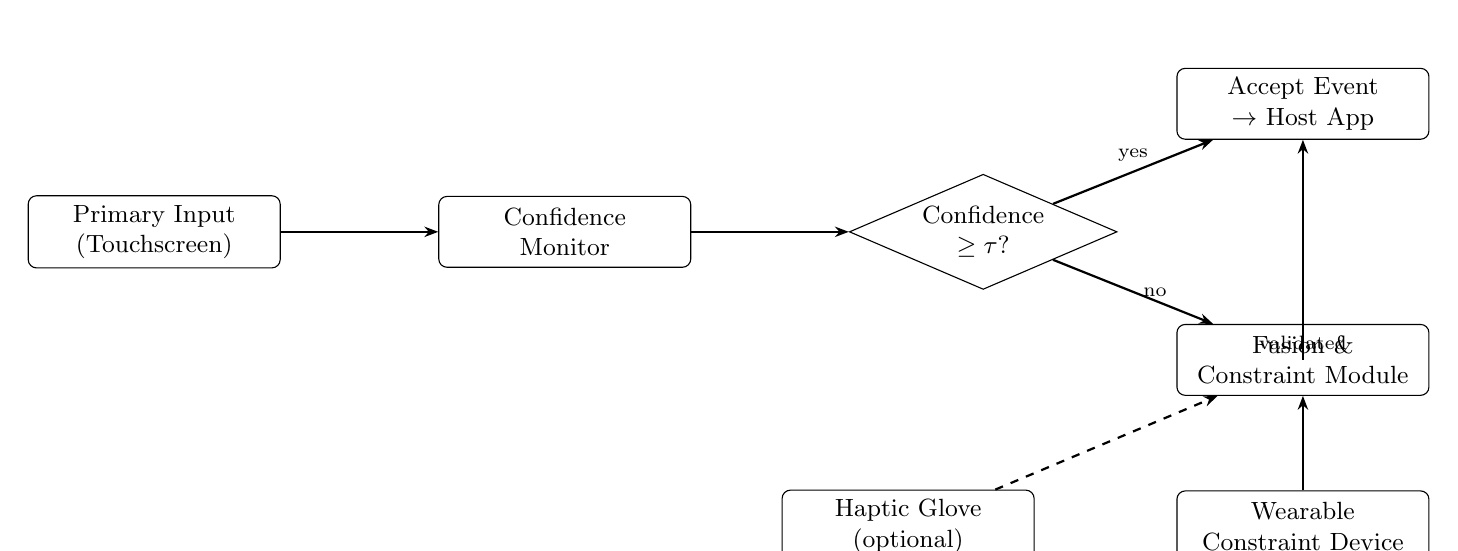
\begin{tikzpicture}[
  node distance = 1.4cm and 2.0cm,
  box/.style = {rectangle, draw, rounded corners=3pt,
                minimum width=3.2cm, minimum height=0.9cm,
                font=\small, align=center},
  decision/.style = {diamond, draw, aspect=2.2,
                     minimum width=3.4cm, minimum height=0.9cm,
                     font=\small, align=center, inner sep=1pt},
  arr/.style = {-{Stealth[length=5pt]}, thick},
  dasharr/.style = {-{Stealth[length=5pt]}, thick, dashed},
]

\node[box] (screen)    {Primary Input\\(Touchscreen)};
\node[box, right=of screen] (monitor)  {Confidence\\Monitor};
\node[decision, right=of monitor] (decision) {Confidence\\$\geq \tau$?};
\node[box, above right=0.8cm and 1.6cm of decision] (accept) {Accept Event\\$\rightarrow$ Host App};
\node[box, below right=0.8cm and 1.6cm of decision] (fusion) {Fusion \&\\Constraint Module};
\node[box, below=1.2cm of fusion] (glasses) {Wearable\\Constraint Device};
\node[box, left=1.8cm of glasses] (gloves) {Haptic Glove\\(optional)};

\draw[arr] (screen)   -- (monitor);
\draw[arr] (monitor)  -- (decision);
\draw[arr] (decision) -- node[above, font=\scriptsize]{yes} (accept);
\draw[arr] (decision) -- node[right, font=\scriptsize]{no} (fusion);
\draw[arr] (glasses)  -- (fusion);
\draw[dasharr] (gloves) -- (fusion);
\draw[arr] (fusion)   -| node[above, font=\scriptsize, pos=0.3]{validated} (accept);

\end{tikzpicture}
\caption{High-level system architecture. Dashed line indicates optional channel.
         The wearable constraint device is activated only when confidence falls
         below threshold $\tau$.}
\label{fig:arch}
\end{figure}

\subsection{Primary Input Device}

The primary input device comprises a mutual-capacitance sensing grid, a touch-event
detection module, and a spatial-temporal signal-processing unit. The device produces
a stream of candidate input events:
\[
  \mathcal{E} = \bigl\{\, e_i = (x_i,\, y_i,\, t_i,\, s_i,\, \sigma_i) \bigr\}
\]
where $(x_i, y_i)$ denotes screen coordinates, $t_i$ the detection timestamp, $s_i$
the integrated signal strength, and $\sigma_i$ a per-event confidence score computed
from signal morphology, contact-area distribution, approach velocity (where
derivable), and historical false-positive rate under current environmental conditions.

The confidence score $\sigma_i \in [0,1]$ is produced by a local classifier trained
on labelled examples of intentional touch, raindrop impact, palm contact, vibrational
artefact, and conductive contamination. Under normal operating conditions the vast
majority of events will have $\sigma_i \geq \tau$, where $\tau$ is the current
acceptance threshold, and will proceed directly to the host application without
consulting any auxiliary channel.

\subsection{Confidence Monitor and Threshold Adaptation}

The confidence monitor maintains a sliding-window estimate of the ambient
false-positive rate $\hat{f}(t)$ and a global environmental state vector
$\mathbf{e}(t)$ incorporating readings from the device's onboard sensors: barometric
pressure, accelerometer, gyroscope, and optionally a dedicated moisture detector at
the screen perimeter.

The acceptance threshold is adapted as:
\[
  \tau(t) = \tau_0 + \alpha \cdot \hat{f}(t) + \beta \cdot v(t)
\]
where $\tau_0$ is a baseline threshold, $v(t)$ is the RMS vibration magnitude from
the accelerometer, and $\alpha, \beta$ are tunable weights. Under calm, dry conditions
$\tau(t) \approx \tau_0$ and auxiliary channels are rarely or never invoked. Under
rain or vibration, $\tau(t)$ rises, causing more events to be held pending
cross-modal confirmation.

The confidence monitor also emits an \emph{activation signal} $A(t) \in \{0,1\}$
transmitted to the secondary wearable device. When $A(t) = 0$, the wearable enters
a low-power idle state. When $A(t) = 1$, the wearable activates its sensing pipeline.
This ensures the wearable consumes negligible power during normal operation.

\subsection{Secondary Wearable Constraint Device}

\subsubsection{Physical Form Factor}

The preferred embodiment of the secondary device takes the form of lightweight
glasses. Alternative embodiments include a headband, an ear-mounted device, or a
shoulder-mounted sensor. The common requirement across all embodiments is that the
device provides a viewpoint geometrically distinct from the primary screen---one from
which the user's hands and the screen surface are simultaneously observable---without
requiring direct line-of-sight from the screen itself.

\subsubsection{Sensing Hardware}

The device comprises one or more of the following sensing modalities:

\begin{itemize}[leftmargin=2em]
  \item A monocular or stereo RGB or monochrome optical sensor.
  \item An infrared illuminator and corresponding IR sensor, enabling operation in
        low-light environments without visible light emission.
  \item A time-of-flight (ToF) depth sensor providing per-pixel range estimates.
  \item An inertial measurement unit (IMU) for head-pose estimation.
\end{itemize}

\subsubsection{Principled Incapacity}

The device is architecturally constrained to prevent recording, storage, and display.
Specifically:

\begin{enumerate}[leftmargin=2em, label=\alph*.]
  \item No non-volatile storage is present. Raw sensor data is processed in working
        memory and discarded within a bounded time window, not to exceed 500
        milliseconds.
  \item No display surface, projector, or optical combiner is present.
  \item The communication interface transmits only derived constraint signals---hand
        position, velocity, finger-extension estimates, and postural-context
        flags---not raw imagery or depth maps.
  \item Hardware attestation mechanisms, implemented in a secure element, certify
        to paired devices that no recording capability is present and that all
        transmitted data conforms to the derived-signal specification.
\end{enumerate}

These constraints are enforced at the hardware level, not merely at the software
level, so that the absence of recording is verifiable rather than merely asserted.

\subsubsection{Constraint Signal}

The wearable produces a constraint signal stream:
\[
  \mathcal{C} = \bigl\{\, c_j = (\mathbf{p}_j,\, \mathbf{v}_j,\, \phi_j,\, t_j,\,
  \psi_j) \bigr\}
\]
where $\mathbf{p}_j$ is the estimated 3-D position of the fingertip in a shared
coordinate frame, $\mathbf{v}_j$ is its velocity vector, $\phi_j$ is the
finger-extension confidence (0 = fully retracted, 1 = fully extended), $t_j$ is the
timestamp, and $\psi_j$ is a postural-context flag encoding whether the user's hands
are in a configuration favourable for deliberate input (see \S\ref{sec:posture}).

\subsection{Fusion and Constraint Evaluation Module}

\subsubsection{Admissibility Function}

The fusion module evaluates held candidate events against the constraint stream. An
event $e_i$ is admitted if and only if:
\[
  A(e_i, \mathcal{C}) = 1
\]
where the admissibility function $A$ is defined as the conjunction of three conditions:

\paragraph{Temporal correlation.}
There exists a constraint observation $c_j \in \mathcal{C}$ such that
$|t_i - t_j| \leq \Delta t$, where $\Delta t$ is a configurable temporal window
(default: 120\,ms).

\paragraph{Spatial intersection.}
The projected screen-plane position of $\mathbf{p}_j$ lies within a tolerance
radius $r$ of $(x_i, y_i)$ in screen coordinates (default: $r = 8\,\mathrm{mm}$).

\paragraph{Motor plausibility.}
The velocity profile $\mathbf{v}_j$ and finger-extension sequence leading to $c_j$
are consistent with a voluntary reach-and-contact motion, as assessed by a
lightweight kinematic classifier. Criteria include: approach velocity within the
range $[v_{\min}, v_{\max}]$ characteristic of deliberate finger contact, monotonic
decrease in finger-to-screen distance over the preceding window, and absence of
lateral scatter inconsistent with directed motion.

Events failing any condition are rejected. Events satisfying all three are promoted
to the host application as validated input.

\subsubsection{Rejection Taxonomy}

Rejected events fall into distinguishable classes:

\begin{itemize}[leftmargin=2em]
  \item \emph{Environmental noise}: events with no temporally proximate constraint
        observation (e.g., raindrops, condensation).
  \item \emph{Vibrational artefacts}: events with coincident constraint observations
        but lacking motor plausibility (e.g., involuntary contact caused by device
        vibration).
  \item \emph{Non-directed contact}: events with a present hand but lacking directed
        approach (e.g., palm resting on screen edge).
\end{itemize}

This taxonomy is retained in an ephemeral in-memory log for adaptive threshold
tuning. The log is not persisted beyond the current interaction session.

\subsection{Postural Context Assessment}
\label{sec:posture}

The postural-context flag $\psi_j$ encodes conditions under which haptic-glove input
is reliable. The wearable assesses postural context by estimating:

\begin{enumerate}[leftmargin=2em, label=\arabic*.]
  \item \emph{Hand elevation}: whether the user's hands are raised to a position
        consistent with active typing or gesture input, as opposed to hanging at the
        sides.
  \item \emph{Gaze alignment}: whether head pose, as estimated from the IMU,
        is directed toward the expected input region. This estimate is coarse and
        does not require eye tracking.
  \item \emph{Stability}: whether hand and head motion are below a vibration
        threshold indicating a stable input posture.
\end{enumerate}

$\psi_j = 1$ when all three conditions are met; $\psi_j = 0$ otherwise. The haptic
glove input channel is enabled only when $\psi_j = 1$, preventing spurious
glove-input events from being generated when the user is walking, gesturing
conversationally, or otherwise not in an input posture.

\subsection{Tertiary Haptic Glove Input Channel}

\subsubsection{Overview}

Haptic gloves encode finger flexion, extension, and contact events as symbolic
input. They do not require physical contact with a screen surface and thus extend
the input modality to environments where screen contact is impractical: standing,
outdoor use with bulky gloves, or hands-full scenarios where only one hand is free.

\subsubsection{Integration with Constraint Framework}

The haptic glove channel participates in the same constraint framework as touch
events. Glove-generated events are treated as candidate inputs and are subject to
postural-context gating via $\psi_j$. A virtual keyboard or gesture vocabulary is
anchored to the user's physical configuration as assessed by the wearable, so that
the mapping between finger motion and intended symbol remains stable as long as
$\psi_j = 1$.

When posture degrades ($\psi_j \to 0$), the glove channel is suspended rather than
continuing to generate potentially incorrect input. This is the key distinction from
prior air-typing systems, which either ignore postural context entirely or require
explicit user activation and deactivation.

\subsubsection{Motor Adaptation}

Over time the fusion module accumulates statistics on the user's characteristic
approach angles, velocities, and inter-key timing. A personalised motor model
$\mathcal{M}_u$ is maintained in local, encrypted storage on the host device (not
the wearable). This model progressively tightens the admissible region for each
user's input events, reducing false positives and increasing recognition accuracy
for that user's specific motor signature. The model is device-local and is not
transmitted.

\subsection{Operational Modes}

\subsubsection{Normal Mode}

The touchscreen operates conventionally. No wearable communication occurs. The
wearable is in low-power idle. All candidate events have $\sigma_i \geq \tau(t)$
and are forwarded directly to the host application. This is the predominant
operational mode.

\subsubsection{Rain and Moisture Rejection Mode}

Activated when the moisture detector or the accelerometer pattern indicates wet
conditions, or when $\hat{f}(t)$ exceeds a moisture-onset threshold. In this mode:

\begin{itemize}[leftmargin=2em]
  \item $\tau(t)$ is elevated.
  \item The wearable is activated.
  \item Touch events require cross-modal confirmation before being admitted.
  \item Events with no temporally proximate constraint observation are discarded.
\end{itemize}

The user experiences transparent operation: the screen continues to respond to
deliberate touches while ignoring raindrops, at the cost of a modest ($\leq$
120\,ms) confirmation latency for events that require cross-modal validation.

\subsubsection{Vibration Rejection Mode}

Activated when accelerometer RMS exceeds a vibration threshold, as occurs on trains,
aircraft, or during earthquakes. In this mode:

\begin{itemize}[leftmargin=2em]
  \item $\tau(t)$ is elevated by the $\beta \cdot v(t)$ term.
  \item The wearable is activated.
  \item Motor plausibility filtering is applied with tightened velocity bounds,
        since intentional touch approaches during vibration have distinctive profiles
        (the user braces and reaches deliberately) distinguishable from vibration-
        induced artefacts (which lack directed approach trajectories).
\end{itemize}

\subsubsection{Glove and Indirect Contact Mode}

Activated when $s_i$ (signal strength) falls below a glove-detection threshold,
indicating a non-conductive or partially conductive contact. In this mode:

\begin{itemize}[leftmargin=2em]
  \item The wearable becomes the primary signal source.
  \item Contact is inferred from finger trajectory rather than surface perturbation.
  \item The screen's electrostatic grid continues to provide coarse positional data
        when available.
\end{itemize}

\subsubsection{Haptic Glove Input Mode}

Activated when haptic gloves are paired and $\psi_j = 1$. The screen may be off or
absent. Symbolic input is generated from glove-encoded finger motion, validated
against the postural-context flag and the user's motor model. When $\psi_j$ drops to
0 (e.g., the user begins walking), this mode is suspended automatically.

\subsection{Calibration and Coordinate Frame Registration}

For spatial-intersection checking, the constraint signal must be expressed in the
same coordinate frame as the screen surface. Calibration is performed at pairing
time and periodically thereafter:

\begin{enumerate}[leftmargin=2em, label=\arabic*.]
  \item The user performs a brief calibration gesture: touching a sequence of
        prompted screen targets.
  \item The fusion module records simultaneous $(x_i, y_i, t_i)$ tuples from the
        screen and $(\mathbf{p}_j, t_j)$ tuples from the wearable.
  \item A rigid-body transform $T: \mathbb{R}^3 \to \mathbb{R}^2$ is estimated by
        least-squares minimisation over the calibration pairs.
  \item The transform is stored on the host device and updated incrementally as
        new validated events accumulate, accommodating slow drift due to changes
        in wearable fit or device position.
\end{enumerate}

\subsection{Communication Interface}

The wearable communicates with the host device via a low-latency wireless protocol
(e.g., Bluetooth Low Energy with a custom constraint-data profile, or Ultra-Wideband
for sub-centimetre ranging). The protocol transmits only the derived constraint
signal $\mathcal{C}$; no raw imagery is transmitted at any time.

End-to-end latency from wearable sensor capture to constraint-signal receipt at the
host device is targeted at $\leq 30\,\mathrm{ms}$, leaving adequate margin within
the 120\,ms temporal window for reliable correlation.

% ============================================================
%  PRIOR ART CONSIDERATIONS
% ============================================================
\section{Prior Art Considerations}

\subsection{Capacitive Touchscreen Filtering}

Single-surface filtering and threshold-adjustment approaches (including ``wet touch''
and ``glove modes'' found in existing devices) cannot resolve the fundamental
underdetermination problem: environmental stimuli and intentional contacts can be
identical at the sensing surface. The present invention differs by introducing an
independent sensing modality whose observations cannot be mimicked by rain or
vibration, transforming the problem from signal classification to cross-modal
constraint satisfaction.

\subsection{Stylus-Based Input}

Active styluses constrain input by requiring a specialised tool with identifiable
characteristics. The present invention generalises constraint enforcement to natural
hand interaction without requiring a dedicated contact instrument, and additionally
addresses environmental noise, which stylus approaches do not.

\subsection{Optical Gesture Recognition}

Prior gesture-recognition systems are designed as primary input modalities and
depend on continuous scene capture. The present invention uses optical sensing as a
secondary constraint channel activated only when needed, and its wearable device is
architecturally incapable of producing a persistent scene record.

\subsection{Smart Glasses and AR Systems}

Existing smart-glasses and augmented-reality platforms emphasise display, annotation,
and recording, raising privacy concerns and creating social friction. The present
invention defines a device class whose distinguishing feature is the principled
\emph{absence} of display and recording capability. This is not a software policy
but a hardware constraint, verifiable through attestation.

\subsection{Swype-Style Gesture Disambiguation}

The Swype input method resolves underdetermined gesture trajectories by projecting
candidate paths into a constrained linguistic space (the user's lexicon), selecting
the interpretation most consistent with language statistics. The present invention
employs a structurally analogous strategy at a lower level of the input stack:
rather than disambiguating which symbol a trajectory encodes, it disambiguates
whether a surface event encodes any intentional act at all. The constraint is
physical and postural rather than linguistic, but the underlying principle---that
raw input is not trusted on its own and must be brought into agreement with an
independent constraint source---is shared.

\subsection{Mobile Sensor Fusion}

Existing sensor-fusion techniques in mobile devices combine co-located sensors
(accelerometer, gyroscope, proximity, barometric pressure). The present invention
extends sensor fusion across physically separate devices, incorporating an
external wearable viewpoint, which is a qualitatively distinct extension not
achieved by prior intra-device approaches.

\subsection{Air-Typing and Haptic Glove Systems}

Prior haptic and air-typing systems operate independently of touch interfaces and
do not incorporate postural-context gating. The present invention integrates haptic
input as one channel within a unified constraint framework and explicitly gates
glove-mode activation on a postural-context assessment derived from the wearable,
preventing spurious input during ambiguous body configurations.

% ============================================================
%  CLAIMS
% ============================================================
\section{Claims}

\setcounter{claimnum}{0}

\claim{A system for multimodal input disambiguation comprising: a primary input
device including a capacitive touchscreen and a signal-processing unit configured to
produce a stream of candidate input events with associated confidence scores; a
confidence monitor configured to compute a per-event confidence score and to compare
said score to a dynamically adjusted acceptance threshold; and a secondary wearable
constraint device configured to produce real-time constraint signals encoding hand
position, velocity, and motor plausibility, wherein said secondary device is
activated only when said confidence monitor determines that the primary-signal
confidence is insufficient.}

\claim{The system of claim~1, wherein the secondary wearable constraint device is
architecturally incapable of storing persistent imagery or video data, transmitting
raw sensor imagery, or providing a visual display surface.}

\claim{The system of claim~2, wherein the secondary wearable constraint device
includes a hardware attestation mechanism that certifies to a paired host device
that no recording capability is present and that all transmitted data conforms to a
derived-signal specification.}

\claim{The system of claim~1, wherein a candidate input event is promoted to the
host application if and only if there exists a constraint observation satisfying
temporal correlation within a configurable window, spatial intersection within a
tolerance radius in screen coordinates, and motor plausibility as assessed by a
kinematic classifier.}

\claim{The system of claim~1, wherein the acceptance threshold is adapted as a
function of estimated ambient false-positive rate and RMS vibration magnitude, such
that the threshold increases under rain or mechanical vibration.}

\claim{The system of claim~1, wherein the secondary wearable constraint device is
placed in a low-power idle state when the confidence monitor determines that
primary-signal confidence is sufficient, and is activated by an explicit signal from
the confidence monitor when the threshold is exceeded.}

\claim{The system of claim~1, further comprising a tertiary haptic glove input
device, wherein glove-generated input events are subject to a postural-context gate
derived from the secondary wearable constraint device, such that glove-mode input is
enabled only when the user's hands, head orientation, and motion magnitude satisfy
predefined postural-context criteria.}

\claim{The system of claim~7, wherein the postural-context gate assesses hand
elevation, coarse gaze alignment estimated from an inertial measurement unit, and
hand-motion stability, and wherein glove-mode input is automatically suspended when
any postural-context criterion is not met.}

\claim{The system of claim~1, wherein a coordinate-frame registration transform is
estimated from simultaneous paired observations of calibration touch events and
corresponding wearable constraint observations, and is updated incrementally as
validated events accumulate during normal operation.}

\claim{The system of claim~1, wherein rejected candidate events are classified into
an ephemeral in-memory rejection taxonomy comprising environmental noise,
vibrational artefacts, and non-directed contact, and wherein said taxonomy informs
adaptive threshold adjustment without being persisted beyond the current interaction
session.}

\claim{The system of claim~1, wherein a personalised motor model is maintained in
local encrypted storage on the host device and progressively refines the admissible
kinematic region for individual user input events, improving recognition accuracy
over time without transmitting user data to external systems.}

\claim{A method for opportunistic multimodal input disambiguation comprising:
generating candidate input events from a primary capacitive touchscreen;
computing a confidence score for each event; comparing each confidence score to an
adaptive threshold; forwarding events whose confidence meets or exceeds the threshold
directly to the host application; activating a secondary non-recording wearable
sensor upon detecting that confidence is insufficient; receiving constraint signals
from the secondary sensor encoding hand position, velocity, and motor plausibility;
and admitting or rejecting held candidate events based on cross-modal agreement
between screen signals and constraint signals.}

\claim{The method of claim~12, wherein activating the secondary sensor comprises
transmitting an explicit activation signal to a wearable device that was previously
in a low-power idle state, such that the wearable consumes negligible power during
normal operation.}

\claim{The method of claim~12, further comprising assessing postural context from
the secondary sensor and enabling a haptic glove input channel only when the assessed
postural context satisfies predefined criteria.}

\claim{A wearable constraint device comprising: an optical or infrared sensor;
an on-device processing unit configured to estimate hand position, velocity, and
finger-extension state from transient sensor data; a communication interface
configured to transmit derived constraint signals to a paired host device; and
hardware limitations that prevent persistent storage of sensor imagery, raw data
transmission, and visual display output, wherein the device is designed to serve
as an ephemeral constraint provider for touch-input disambiguation rather than as
a primary input, display, or recording device.}

% ============================================================
%  ABSTRACT OF THE DISCLOSURE
% ============================================================
\section*{Brief Description of the Drawings}

\textbf{Figure~1} is a block diagram illustrating the high-level architecture of the
system, including the primary input device, confidence monitor, fusion module,
wearable constraint device, and optional haptic glove channel.

Additional figures, including a timing diagram for opportunistic activation, a
spatial-intersection schematic for coordinate-frame registration, and a postural-
context state diagram, are contemplated for a non-provisional filing.

% ============================================================
%  THEORETICAL FRAMING (OPTIONAL APPENDIX)
% ============================================================
\section*{Appendix: Theoretical Framing}

The invention can be situated within a broader theory of \emph{constraint-enforced
input systems}. In this framing, a touchscreen operating alone attempts to infer
intentional input from a single recurrence channel: repeated perturbations of an
electrostatic field. The problem is that the field cannot distinguish the sources
of perturbation. The invention resolves this by coupling the primary recurrence
channel to a secondary constraint channel, so that an input event is admitted only
when it satisfies the structure imposed by both.

This is structurally analogous to Swype-style keyboard input, in which a raw gesture
trajectory is disambiguated by projecting it into a constrained linguistic space. The
present invention performs an analogous disambiguation at the level of physical
plausibility rather than symbolic identity: instead of asking \emph{which word does
this trajectory encode}, it asks \emph{does this surface event encode any deliberate
act at all}. The constraint is physical and kinematic rather than lexical, but the
structural principle is the same: raw signals are not trusted in isolation; they must
agree with an independent constraint before being admitted.

The device itself embodies a corresponding design principle. Smart glasses fail
partly because they are underspecified: users and bystanders cannot determine what
they are doing. The wearable device described herein is overspecified in the opposite
direction---it is defined as much by what it cannot do as by what it can. A device
whose architectural incapacities are verifiable through hardware attestation occupies
a different social category from a general-purpose recording device. It is legible
in the way that a keyboard, mouse, or stylus is legible: its function is narrow,
its operation is transient, and it produces no durable record of the world.

\vspace{24pt}
\hrule
\vspace{8pt}
\noindent\small\textit{This document constitutes a draft patent specification
prepared for conceptual documentation purposes under the Canadian Patent Act,
R.S.C.\ 1985, c.~P-4. It has not been filed with the Canadian Intellectual Property
Office (CIPO) and confers no legal priority date. A formal application may be filed
with CIPO at any time prior to public disclosure to establish priority. All technical
specifications are subject to revision. The inventor is resident in Canada.}

\end{document}
